\section{Referencia de la Clase List\-Descuento\-Presupuesto}
\label{classListDescuentoPresupuesto}\index{ListDescuentoPresupuesto@{ListDescuentoPresupuesto}}
Muestra y administra la lista de descuentos por presupuesto.  


{\tt \#include $<$listdescpresupuesto.h$>$}

Diagrama de colaboraci\'{o}n para List\-Descuento\-Presupuesto:\begin{figure}[H]
\begin{center}
\leavevmode
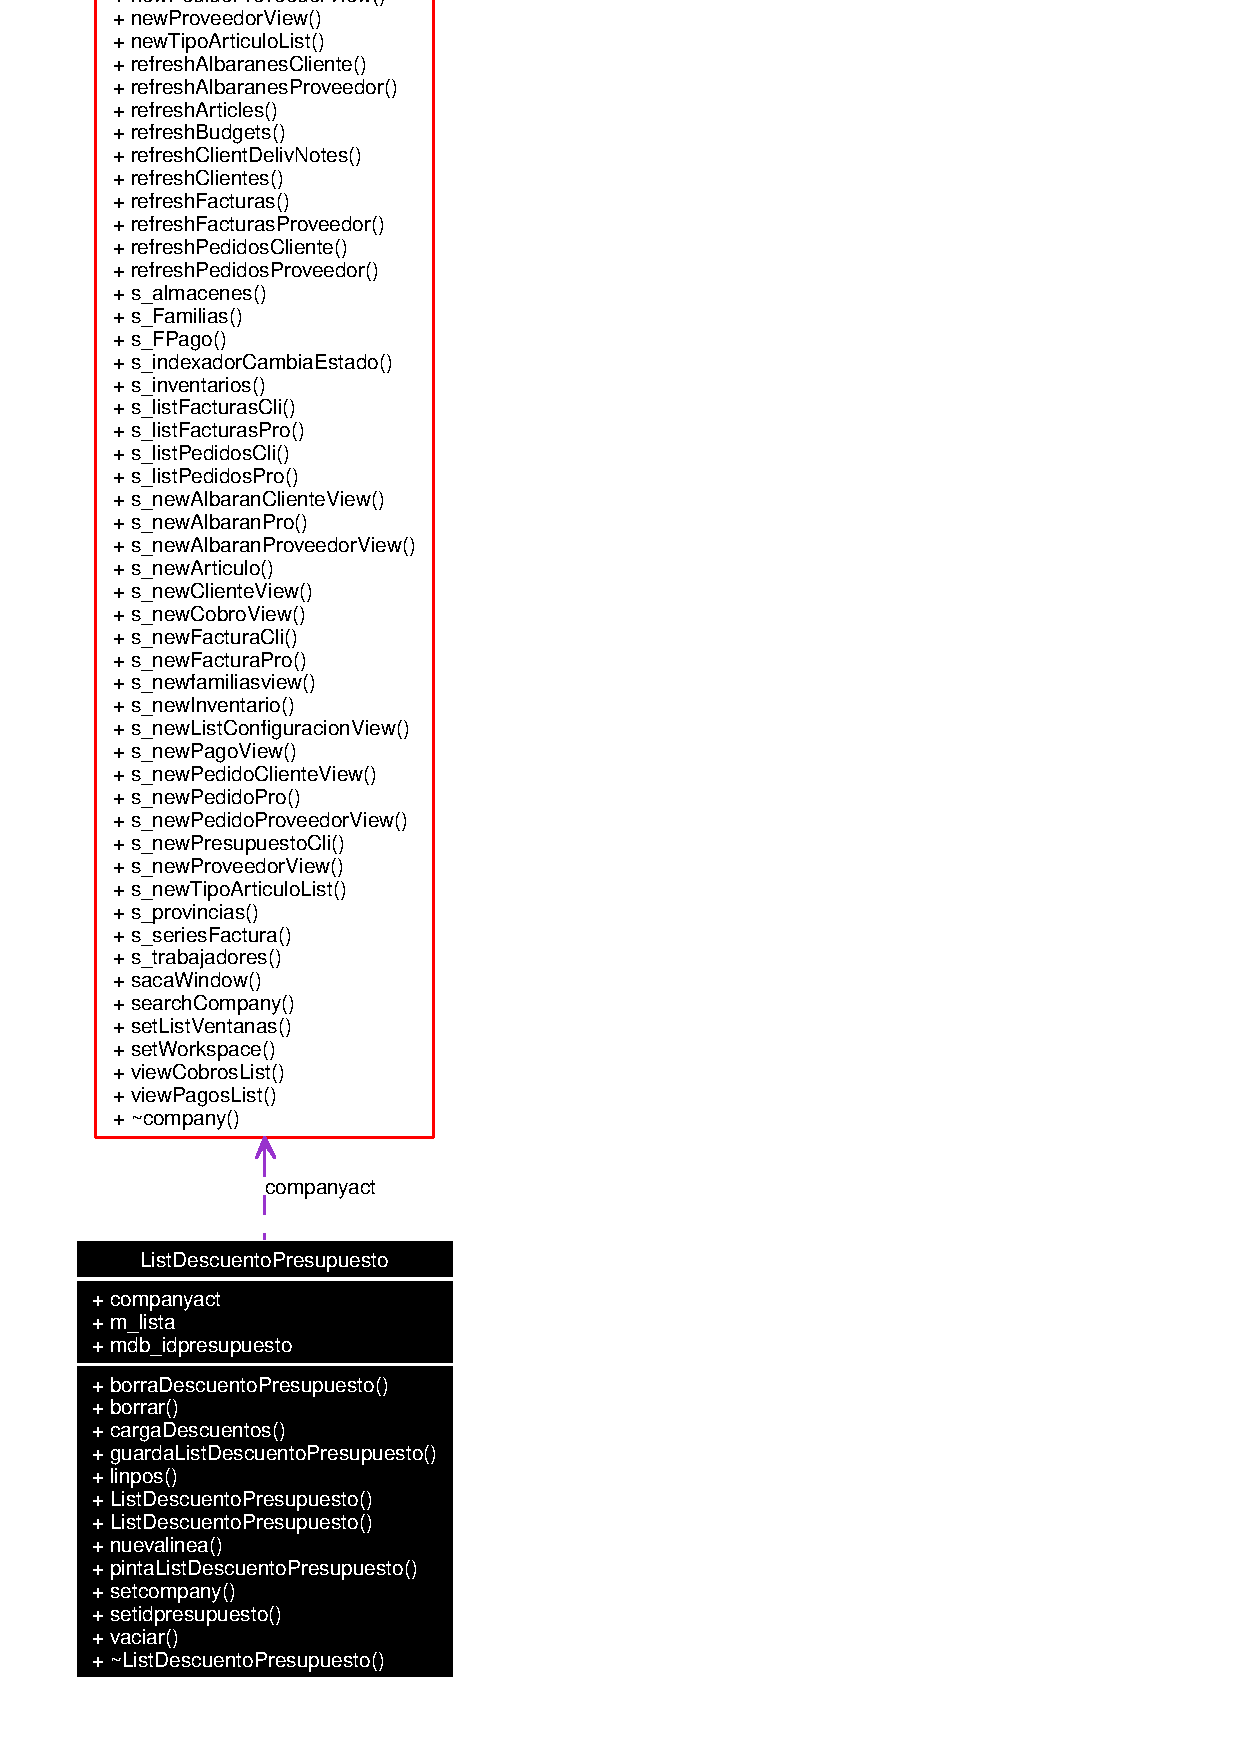
\includegraphics[width=109pt]{classListDescuentoPresupuesto__coll__graph}
\end{center}
\end{figure}
\subsection*{M\'{e}todos p\'{u}blicos}
\begin{CompactItemize}
\item 
int {\bf borra\-Descuento\-Presupuesto} (int)\label{classListDescuentoPresupuesto_a0}

\item 
int {\bf borrar} ()\label{classListDescuentoPresupuesto_a1}

\item 
int {\bf carga\-Descuentos} (QString)
\begin{CompactList}\small\item\em Carga lineas de presupuesto. \item\end{CompactList}\item 
void {\bf guarda\-List\-Descuento\-Presupuesto} ()\label{classListDescuentoPresupuesto_a3}

\item 
{\bf Descuento\-Presupuesto} $\ast$ {\bf linpos} (int)\label{classListDescuentoPresupuesto_a4}

\item 
{\bf List\-Descuento\-Presupuesto} ({\bf company} $\ast$comp)\label{classListDescuentoPresupuesto_a6}

\item 
void {\bf nuevalinea} (QString concept, QString propor)\label{classListDescuentoPresupuesto_a7}

\item 
virtual void {\bf pinta\-List\-Descuento\-Presupuesto} ()\label{classListDescuentoPresupuesto_a8}

\item 
void {\bf setcompany} ({\bf company} $\ast$c)\label{classListDescuentoPresupuesto_a9}

\item 
void {\bf setidpresupuesto} (QString id)\label{classListDescuentoPresupuesto_a10}

\item 
void {\bf vaciar} ()\label{classListDescuentoPresupuesto_a11}

\end{CompactItemize}
\subsection*{Atributos p\'{u}blicos}
\begin{CompactItemize}
\item 
{\bf company} $\ast$ {\bf companyact}\label{classListDescuentoPresupuesto_o0}

\item 
QList$<$ {\bf Descuento\-Presupuesto} $\ast$ $>$ {\bf m\_\-lista}\label{classListDescuentoPresupuesto_o1}

\item 
QString {\bf mdb\_\-idpresupuesto}\label{classListDescuentoPresupuesto_o2}

\end{CompactItemize}


\subsection{Descripci\'{o}n detallada}
Muestra y administra la lista de descuentos por presupuesto. 



\subsection{Documentaci\'{o}n de las funciones miembro}
\index{ListDescuentoPresupuesto@{List\-Descuento\-Presupuesto}!cargaDescuentos@{cargaDescuentos}}
\index{cargaDescuentos@{cargaDescuentos}!ListDescuentoPresupuesto@{List\-Descuento\-Presupuesto}}
\subsubsection{\setlength{\rightskip}{0pt plus 5cm}int List\-Descuento\-Presupuesto::carga\-Descuentos (QString {\em idbudget})}\label{classListDescuentoPresupuesto_a2}


Carga lineas de presupuesto. 

Creamos un elemento del tipo {\bf Descuento\-Presupuesto}{\rm (p.\,\pageref{classDescuentoPresupuesto})} y lo agregamos a la lista.

Tratamiento de excepciones. 

La documentaci\'{o}n para esta clase fu\'{e} generada a partir de los siguientes archivos:\begin{CompactItemize}
\item 
listdescpresupuesto.h\item 
listdescpresupuesto.cpp\end{CompactItemize}
